\documentclass[11pt]{article}
\usepackage[a4paper,margin=2.4cm]{geometry}
\usepackage{booktabs,graphicx,amsmath,hyperref,xcolor}
\hypersetup{colorlinks,linkcolor=blue!50!black,citecolor=blue!50!black,urlcolor=blue!50!black}
\usepackage[numbers,sort&compress]{natbib}

\title{From 1.00 to 0.77:\\
\large How Much of Reported Dementia-Prediction Accuracy on OASIS Is Leakage?}
\author{Mithil Nagabathula\\University of East London\\\texttt{mithilnishu2000@gmail.com}}
\date{October 2026}

\begin{document}
\maketitle
\sloppy

\begin{abstract}
The OASIS longitudinal dataset is a common first benchmark for machine-learning dementia prediction, and tutorials and student projects
routinely report near-perfect accuracy from its tabular summary file. We quantify how much of that accuracy comes from three
protocol choices: using the Clinical Dementia Rating (CDR) as a feature when it defines the label, splitting visits rather than
participants, and including the Mini-Mental State Examination (MMSE), a cognitive test that is close to a diagnosis in itself. With
all three, every model reached an AUC of 1.000. Removing CDR left 0.89--0.91; splitting by participant cost the flexible models six
points (random forest 0.904 to 0.842) but not logistic regression; removing MMSE left demographic and MRI-volume features with AUC
0.67--0.77. On an external cohort (OASIS-1, aged 60 or over) the same feature set reached 0.74--0.88, so internal cross-validation in
150 participants did not predict external performance in either direction. Subgroup AUCs by sex, age and education had confidence
intervals 0.18--0.29 wide, too wide to detect or exclude disparities. A defensible headline for this dataset is ``moderate
discrimination from MRI volumetrics and demographics, uncertain by about 0.15'', not ``99\% accuracy''.
\end{abstract}

\section{Introduction}
Data leakage, where information about the target reaches the model through the features or the split, is a leading cause of
irreproducible machine-learning results \cite{kapoor2023leakage}, and Alzheimer's disease classification has been a documented
example \cite{wen2020ad}. Medical imaging studies more broadly suffer from small samples, optimistic evaluation and unstable subgroup
estimates \cite{varoquaux2022failures}.

The Open Access Series of Imaging Studies (OASIS) releases MRI data together with a tabular summary per scan
\cite{marcus2007oasis,marcus2010oasis2}. The longitudinal OASIS-2 summary has 373 visits from 150 older adults, each with demographics,
socioeconomic status, MMSE \cite{folstein1975mmse}, CDR \cite{morris1993cdr} and three MRI-derived measures: estimated total
intracranial volume (eTIV), normalised whole-brain volume (nWBV) and the atlas scaling factor. It is widely mirrored, and widely used to
teach classification.

Three features of this file invite leakage. The label used in most analyses, ``demented'' or a CDR above zero, is a function of the CDR
column. Participants contribute up to five visits, so a random split of rows puts the same person in training and test sets. And MMSE
is part of the clinical assessment that leads to the diagnosis. We measure the contribution of each, then evaluate the remaining
model externally and by subgroup, following the spirit of TRIPOD+AI \cite{collins2024tripodai}.

\section{Data and methods}
\paragraph{Data.} OASIS-2: 373 visits, 150 participants aged 60--98, 45\% of visits with CDR \(>\) 0 (CDR 0.5: 123; 1: 41; 2: 3); 16
participants change status across visits. External set: OASIS-1 participants aged 60 or over with a CDR rating (198; 51\% CDR \(>\)
0). Years of education in OASIS-2 were mapped to the five OASIS-1 education categories. The target is CDR \(>\) 0 at each visit.

\paragraph{Protocols.} P1: rows split at random (5-fold), all features including CDR. P2: as P1 without CDR. P3: participants split
(grouped 5-fold), with MMSE. P4: participants split, demographics (age, sex, education, SES) and MRI measures only. P5: the P4 feature
set trained on all of OASIS-2 and tested on OASIS-1; P5b adds MMSE. Each protocol was repeated with five seeds.

\paragraph{Models and metrics.} Logistic regression (standardised, median imputation), random forest (200 trees, minimum leaf 3) and
gradient boosting (depth 3). We report AUC, balanced accuracy, Brier score and expected calibration error (ECE). Subgroup AUCs for P4
use out-of-fold predictions with participant-level bootstrap intervals.

\section{Results}
\begin{table*}[t]
\centering
\caption{Dementia (CDR $>$ 0) classification under five protocols, mean of five repetitions. P1--P4 are 5-fold cross-validation on OASIS-2 (373 visits, 150 participants); P5 trains on all of OASIS-2 and tests on OASIS-1 participants aged 60 or over (198).}
\label{tab:protocols}
\small
\begin{tabular}{llrrrr}
\toprule
Protocol & Model & AUC & Bal.\ acc. & Brier & ECE \\
\midrule
P1 visit split, all features incl. CDR & Logistic regression & 1.000 & 1.000 & 0.001 & 0.025 \\
 & Random forest & 1.000 & 1.000 & 0.004 & 0.043 \\
 & Gradient boosting & 1.000 & 1.000 & 0.000 & 0.000 \\
P2 visit split, MMSE, no CDR & Logistic regression & 0.907 & 0.817 & 0.123 & 0.046 \\
 & Random forest & 0.904 & 0.814 & 0.124 & 0.066 \\
 & Gradient boosting & 0.892 & 0.807 & 0.129 & 0.056 \\
P3 subject split, MMSE & Logistic regression & 0.900 & 0.813 & 0.127 & 0.038 \\
 & Random forest & 0.842 & 0.763 & 0.156 & 0.077 \\
 & Gradient boosting & 0.842 & 0.747 & 0.166 & 0.103 \\
P4 subject split, demographics + MRI & Logistic regression & 0.766 & 0.699 & 0.195 & 0.060 \\
 & Random forest & 0.671 & 0.630 & 0.232 & 0.074 \\
 & Gradient boosting & 0.679 & 0.625 & 0.246 & 0.146 \\
P5 external OASIS-1, demographics + MRI & Logistic regression & 0.742 & 0.663 & 0.214 & 0.090 \\
 & Random forest & 0.877 & 0.773 & 0.154 & 0.117 \\
 & Gradient boosting & 0.824 & 0.753 & 0.175 & 0.090 \\
P5b external OASIS-1, + MMSE & Logistic regression & 0.905 & 0.823 & 0.130 & 0.073 \\
 & Random forest & 0.948 & 0.885 & 0.095 & 0.111 \\
 & Gradient boosting & 0.940 & 0.849 & 0.099 & 0.059 \\
\bottomrule
\end{tabular}
\end{table*}


\begin{figure}[t]
  \centering
  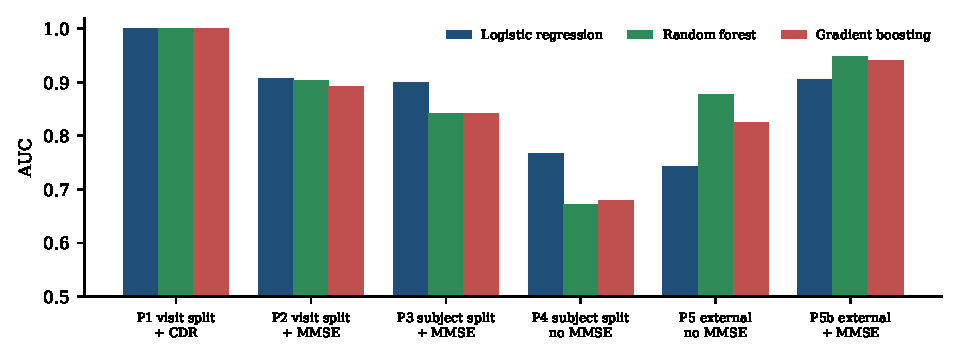
\includegraphics[width=\linewidth]{figures/protocols.pdf}
  \caption{AUC by protocol and model (mean of five repetitions).}
  \label{fig:protocols}
\end{figure}

\paragraph{Target leakage.} With CDR as a feature every model reached AUC 1.000 and balanced accuracy 1.000 (P1,
Table~\ref{tab:protocols}): the model reads the label.

\paragraph{Participant leakage.} Removing CDR but splitting visits (P2) gave AUC 0.89--0.91. Splitting by participant (P3) cost the random
forest 6.2 points (0.904 to 0.842) and gradient boosting 5.0 points (0.892 to 0.842), but logistic regression only 0.7 points (0.907 to
0.900). Flexible models memorise individuals whose other visits are in the training set; a linear model has less capacity to do so. The
ranking of models changed with the protocol.

\paragraph{The cognitive test.} Removing MMSE (P4) cut AUC to 0.766 for logistic regression (participant-bootstrap 95\% CI
0.690--0.840) and to 0.67--0.68 for the tree models. Most of the apparent skill in P2 and P3 is the MMSE score, which is part of the same
clinical assessment that assigns CDR. A model that needs an MMSE to predict a CDR adds little for a clinician who has both.

\paragraph{External validation.} Trained on OASIS-2 and tested on OASIS-1 (P5), the demographic and MRI model reached 0.742 (logistic
regression), 0.824 (gradient boosting) and 0.877 (random forest). Tree models did better externally than in internal cross-validation,
the opposite of the usual pattern. The OASIS-1 set is cross-sectional, one scan per person, with a slightly different mix of severity, and
the tree models were trained on all 373 visits rather than four fifths. Whatever the cause, internal cross-validation in 150
participants did not predict external performance, in either direction.

\begin{table}[t]
\centering
\caption{Subgroup AUC for the P4 logistic-regression model (out-of-fold predictions; participant-level bootstrap CIs).}
\label{tab:sub}
\small
\setlength{\tabcolsep}{4pt}
\begin{tabular}{llrrrr}
\toprule
Group & Level & Visits & Participants & CDR$>$0 & AUC [95\% CI] \\
\midrule
Sex & female & 213 & 88 & 33\% & 0.761 [0.651, 0.845] \\
Sex & male & 160 & 62 & 60\% & 0.714 [0.576, 0.830] \\
Age & 75-84 & 153 & 74 & 46\% & 0.732 [0.607, 0.839] \\
Age & 85+ & 54 & 27 & 35\% & 0.860 [0.686, 0.974] \\
Age & <75 & 166 & 76 & 46\% & 0.780 [0.670, 0.871] \\
Education & beyond high school & 247 & 97 & 36\% & 0.749 [0.650, 0.834] \\
Education & high school or less & 126 & 53 & 61\% & 0.737 [0.599, 0.874] \\
\bottomrule
\end{tabular}
\end{table}


\paragraph{Subgroups.} Table~\ref{tab:sub} gives P4 AUCs by sex, age and education. Point estimates ranged from 0.714 (men) to 0.860
(aged 85 or over), but every interval spanned at least 0.18, and most overlap. With 27--97 participants per subgroup, the dataset
cannot show that the model is fair across these groups, nor that it is not. Base rates also differ sharply (CDR \(>\) 0 in 33\% of
women's visits and 60\% of men's), which affects any threshold-based fairness metric.

\paragraph{Calibration.} Logistic regression stayed reasonably calibrated throughout (ECE 0.03--0.09) and was the best calibrated
model under participant splitting (P3, P4). Tree models' calibration
worsened under participant splitting (gradient boosting ECE 0.056 in P2, 0.103 in P3, 0.146 in P4).

\section{Discussion}
Each of the three choices is easy to make and invisible in the headline number. Together they turn a model with moderate
discrimination into one that appears perfect. The order also matters for teaching: participant leakage is subtle and inflates flexible
models more than linear ones, so a comparison of model families under a row split favours the wrong family.

\paragraph{Recommendations for work with OASIS and similar data.} (1) Never use any feature that defines or is derived from the label.
(2) Split by participant. (3) Decide whether cognitive test scores belong in the model given its intended use, and report results with
and without them. (4) Report external validation, even on a sibling cohort, and expect it to differ. (5) Report subgroup results with
intervals, and say when the sample cannot answer the fairness question.

\paragraph{Limitations.} This is a tabular analysis of summary files, not of images. OASIS-1 and OASIS-2 come from the same research
centre and may share participants; we could not check this from the public files. CDR \(>\) 0 includes very mild impairment (CDR 0.5),
which is a harder and clinically different target from moderate dementia. Five seeds of grouped cross-validation on 150 participants leave
the internal estimates uncertain.

\section{Conclusion}
On OASIS, the path from AUC 1.00 to 0.77 runs through target leakage, participant leakage and a near-diagnostic cognitive test. Honest
evaluation of dementia prediction on this dataset gives moderate discrimination with wide uncertainty, which is the right starting point
for research on better features and larger cohorts.

\paragraph{Reproducibility.} Code and results will be released at
\newline\url{https://github.com/mithil2k2000-tech/oasis-leakage}. The OASIS data are available from the OASIS project under its terms.

\paragraph{Use of AI tools.} An AI assistant (Claude, Anthropic) helped write analysis code and draft text. The author designed the
study, reviewed the code and results, and takes responsibility for the content.

\bibliographystyle{plainnat}
\bibliography{refs}
\end{document}
